\chapter{Testen}
In dit hoofdstuk wordt er gekeken naar de testen die gedaan zijn tijdens het traject, ten eerste wordt er gekeken naar het testplan van de hardware validatie, maar ook het testplan voor de applicatie. Testen in softwareontwikkeling is een belangrijk onderdeel, hiermee kan er goed gekeken hoe robuust de applicatie is geworden.

\section{Testplan hardware validatie} \label{sec:hwtestplan}
Dit is het testplan die bedacht is om de alle porten van de Satellite te testen, dit is testplan die wordt gebruikt bij Satellite hardware. Hiermee kan Sensor Maritime heel snel de hardware verifiëren.
\subsection{DIP switch}
De eerste drie schakelaars worden anders getest in vergelijking met de laatste vier. De laatste vier schakelaars maken vier leds branden die op Satellite zitten. In de volgende tabel \ref{tab:hw_val_dip_testplan} is een overzicht van het testplan:
\begin{table}[h!]
	\caption{DIP switch porten testplan}
	\begin{tabular}{lp{14.5cm}}
	\toprule
	\textbf{Naam} 	& \textbf{Verwachte resultaat} \\ \toprule
	PU1				& Als het aan gezet wordt de range van de analoge input 1 verhoogt naar 24 volt, dit verhoogt de waarde wat de microcontroller leest, de waarde wordt laten zien op een GUI.\\
	-				& Wordt niet getest. \\
	PU2				& Als het aan gezet wordt de range van de analoge input 2 verhoogt naar 24 volt, dit verhoogt de waarde wat de microcontroller leest, de waarde wordt laten zien op een GUI.\\
	PU3				& Als het aan gezet wordt de range van de analoge input 3 verhoogt  naar 24 volt, dit verhoogt de waarde wat de microcontroller leest, de waarde wordt laten zien op een GUI. \\
	ADD0 			& Zet 3.3V op de pin van de microcontroller, als de microcontroller 3.3V detecteert zet het led 0 aan.\\
	ADD1 			& Zet 3.3V op de pin van de microcontroller, als de microcontroller 3.3V detecteert zet het led 1 aan.\\
	ADD2 			& Zet 3.3V op de pin van de microcontroller, als de microcontroller 3.3V detecteert zet het led 2 aan.\\
	ADD3 			& Zet 3.3V op de pin van de microcontroller, als de microcontroller 3.3V detecteert zet het led 3 aan.\\ \bottomrule
	\end{tabular}
	\label{tab:hw_val_dip_testplan}
\end{table}

\newpage
\subsection{Digital output signaal}
Alle digitale output porten voeren dezelfde actie. Het doel is dat als een LED verbonden is met de port dat die dan aan of uit gaat om de 1 seconden.
\begin{table}[h!]
	\caption{Digital output signalen testplan}
	\begin{tabular}{lp{14.5cm}}
	\toprule
	\textbf{Naam} 	& \textbf{Verwachte resultaat} \\ \toprule
	D1	&	Als op de pin 24V staat gaat het lampje aan, en bij 0V uit gaat het uit. Dit gebeurt om 1 seconden. \\			
	D2	&	Als op de pin 24V staat gaat het lampje aan, en bij 0V uit gaat het uit. Dit gebeurt om 1 seconden. \\			
	D3	&	Als op de pin 24V staat gaat het lampje aan, en bij 0V uit gaat het uit. Dit gebeurt om 1 seconden. \\			
	D4	&	Als op de pin 24V staat gaat het lampje aan, en bij 0V uit gaat het uit. Dit gebeurt om 1 seconden. \\ \bottomrule
	\end{tabular}
	\label{tab:hw_val_dio_testplan}
\end{table}

\subsection{Analog input signaal}
Aan de hand wat is beschreven zal er gebruik gemaakt worden van de DIP schakelaars PU1, PU2, en PU3 om de analoge input te testen. De microcontroller heeft een 12 bit Analog to Digital Converter (ADC) \autocite{microcontroller}. Dit betekent dat het bereik van analoge input porten van 0 tot 4096 ($2^{12}$) is. Dus bij 24 volt zal de microcontroller ongeveer 4096 in lezen, het getal kan af en toe lager zijn in verband met ruis. Bij 0 volt zal de microcontroller 0 in lezen. PU1, PU2, PU3 zet het analoge bereik tussen 3,3 volt en 24 volt. Dit betekent als PU1, PU2 of PU3 uitstaan dat de maximale bereik 3,3 volt is en als het aan staat is de bereik 24 Volt. Om het bereik te testen zal er  gemaakt worden van een Graphical User Interface (GUI). De microcontroller zal om 100 microseconden de analoge input omzetten naar een digitale waarden en dit opsturen over UDP. Hiermee kan geverifieerd worden dat als de DIP schakelaars uitstaan dat het bereik van de waarden van 0 tot 1100 gaan. Als de DIP schakelaars aan staan dan zal het bereik zijn van 0 tot 4096. Hieronder is een overzicht van hoe de analoge input porten gevalideerd worden \ref{tab:hw_val_ai_testplan}.
\begin{table}[h!]
	\caption{Testplan voor de analoge input signalen}
	\begin{tabular}{lp{14.5cm}}
	\toprule
	\textbf{Naam} 	& \textbf{Verwachte resultaat} \\ \toprule
	AI1			& Als de schakelaar PU1 van de schakelaar aangezet wordt dan zal de data bereik op de graphical user interface aangepast worden naar 0 tot 4096. Als het dip schakelaar uit staat dan zal de bereik maar van 0 tot 1100 gaan.\\
	AI2			& Als de schakelaar PU1 van de schakelaar aangezet wordt dan zal de data bereik op de graphical user interface aangepast worden naar 0 tot 4096. Als het dip schakelaar uit staat dan zal de bereik maar van 0 tot 1100 gaan.\\
	AI3			& Als de schakelaar PU1 van de schakelaar aangezet wordt dan zal de data bereik op de graphical user interface aangepast worden naar 0 tot 4096. Als het dip schakelaar uit staat dan zal de bereik maar van 0 tot 1100 gaan.\\  \bottomrule
	\end{tabular}
	\label{tab:hw_val_ai_testplan}
\end{table}

\subsection{Relay}
De relay geeft bij het sluiten en het openen van de mechanische connectie een luid geluid die op normale afstand van het apparaat te horen moet zijn. Het testplan van de relay wordt dan ook op geluid gedaan. De relay zal dan voor vijf seconden aan gaan, en vervolgens weer voor vijf seconden uitgaan. Hieronder is een overzicht van de relay testplan \ref{tab:hw_val_relay_testplan}.

\begin{table}[h!]
	\caption{Testplan voor de relay}
	\begin{tabular}{lp{14.5cm}}
	\toprule
	\textbf{Naam} 	& \textbf{Verwachte resultaat} \\ \toprule
	Relay			& De microcontroller zet de pin van de relay voor vijf seconden hoog, als dit gebeurt hoor je een klik te horen. Na vijf seconden zal deze pin weer laag gezet worden, dit moet ook gehoord kunnen worden.\\  \bottomrule
	\end{tabular}
	\label{tab:hw_val_relay_testplan}
\end{table}


\subsection{Serieel communicatie}
Om de seriele communicatie te testen wordt er gebruik gemaakt van GUI. Deze GUI vraagt de om gebruikers input hierin kan de gebruiker een tekst schrijven en dit wordt opgestuurd. De tekst heeft een limiet van maximaal 32 karakters. Er zal hier automatisch een newline karakter toegevoegd worden zodat de microcontroller weet dat dit het einde van het gebruikers bericht is. Het bericht wordt opgestuurd naar de microcontroller en zal de data verwerken. De microcontroller zal dan een antwoord geven als volgt, ten eerste zal de microcontroller vertellen welke variant van communicatie is gebruikt en daarna zal het toevoegen wat de microcontroller ontvangen heeft van de gebruiker. Hieronder is een overzicht \ref{fig:testplanserieel} van hoe het testplan zal werken.

\begin{figure}[h!]
	\centering

	\label{fig:testplanserieel}
	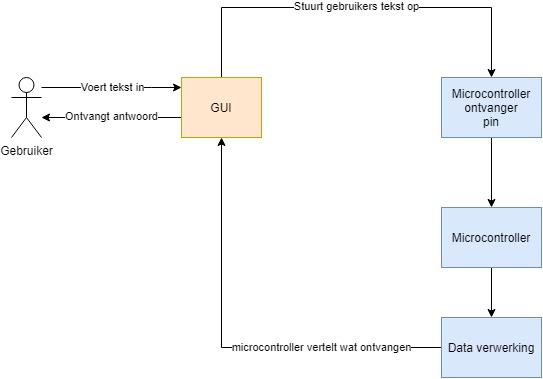
\includegraphics[width=0.5\linewidth]{voorstudie/testplan/Serieel.jpg}
	\caption{Testplan serieel communicatie}
\end{figure}

\newpage

\subsection{GUI}
\section{Applicatie}
De applicatie moet voldoen aan de eisen en doelstelling die bepaald zijn in hoofdstuk \ref{ch:aanpak}, hiervoor is gebruikt gemaakt van twee manieren van testen. Ten eerste wordt er gebruikt gemaakt van een GUI die data ontvangt van de Satellite en toont op GUI in vorm van grafieken en tabellen. Er is hiervoor een nieuw project begonnen die afstudeerder zelf ontwikkeld heeft. De tweede manier van testen is gebruikt maken van de onboard LED's die de Satellite standaard beschikt. De Satellite heeft in totaal vier LED's die softwareontwikkelaar aan of uit kan zetten. 



\subsection{GUI}
Om de applicatie te testen is er gebruik gemaakt van een desktopapplicatie die alle data ontvangt en visualiseert in verschillende grafieken. Dit geeft de gebruiker direct input of een applicatie werkt na toebehoren. Er is voor elke sensor een nieuw tabblad gemaakt waarop dat weergeeft wordt. Om de applicatie goed te testen is dan ook de applicatie gebruikt op lange termijn zodat de softwareontwikkelaar ook weet of het over drie uur nog steeds zal werken. Hieronder is een voorbeeld \ref{fig:guitest} hoe de user interface eruitziet. 
\begin{figure}[h!]
	\centering

	\label{fig:guitest}
	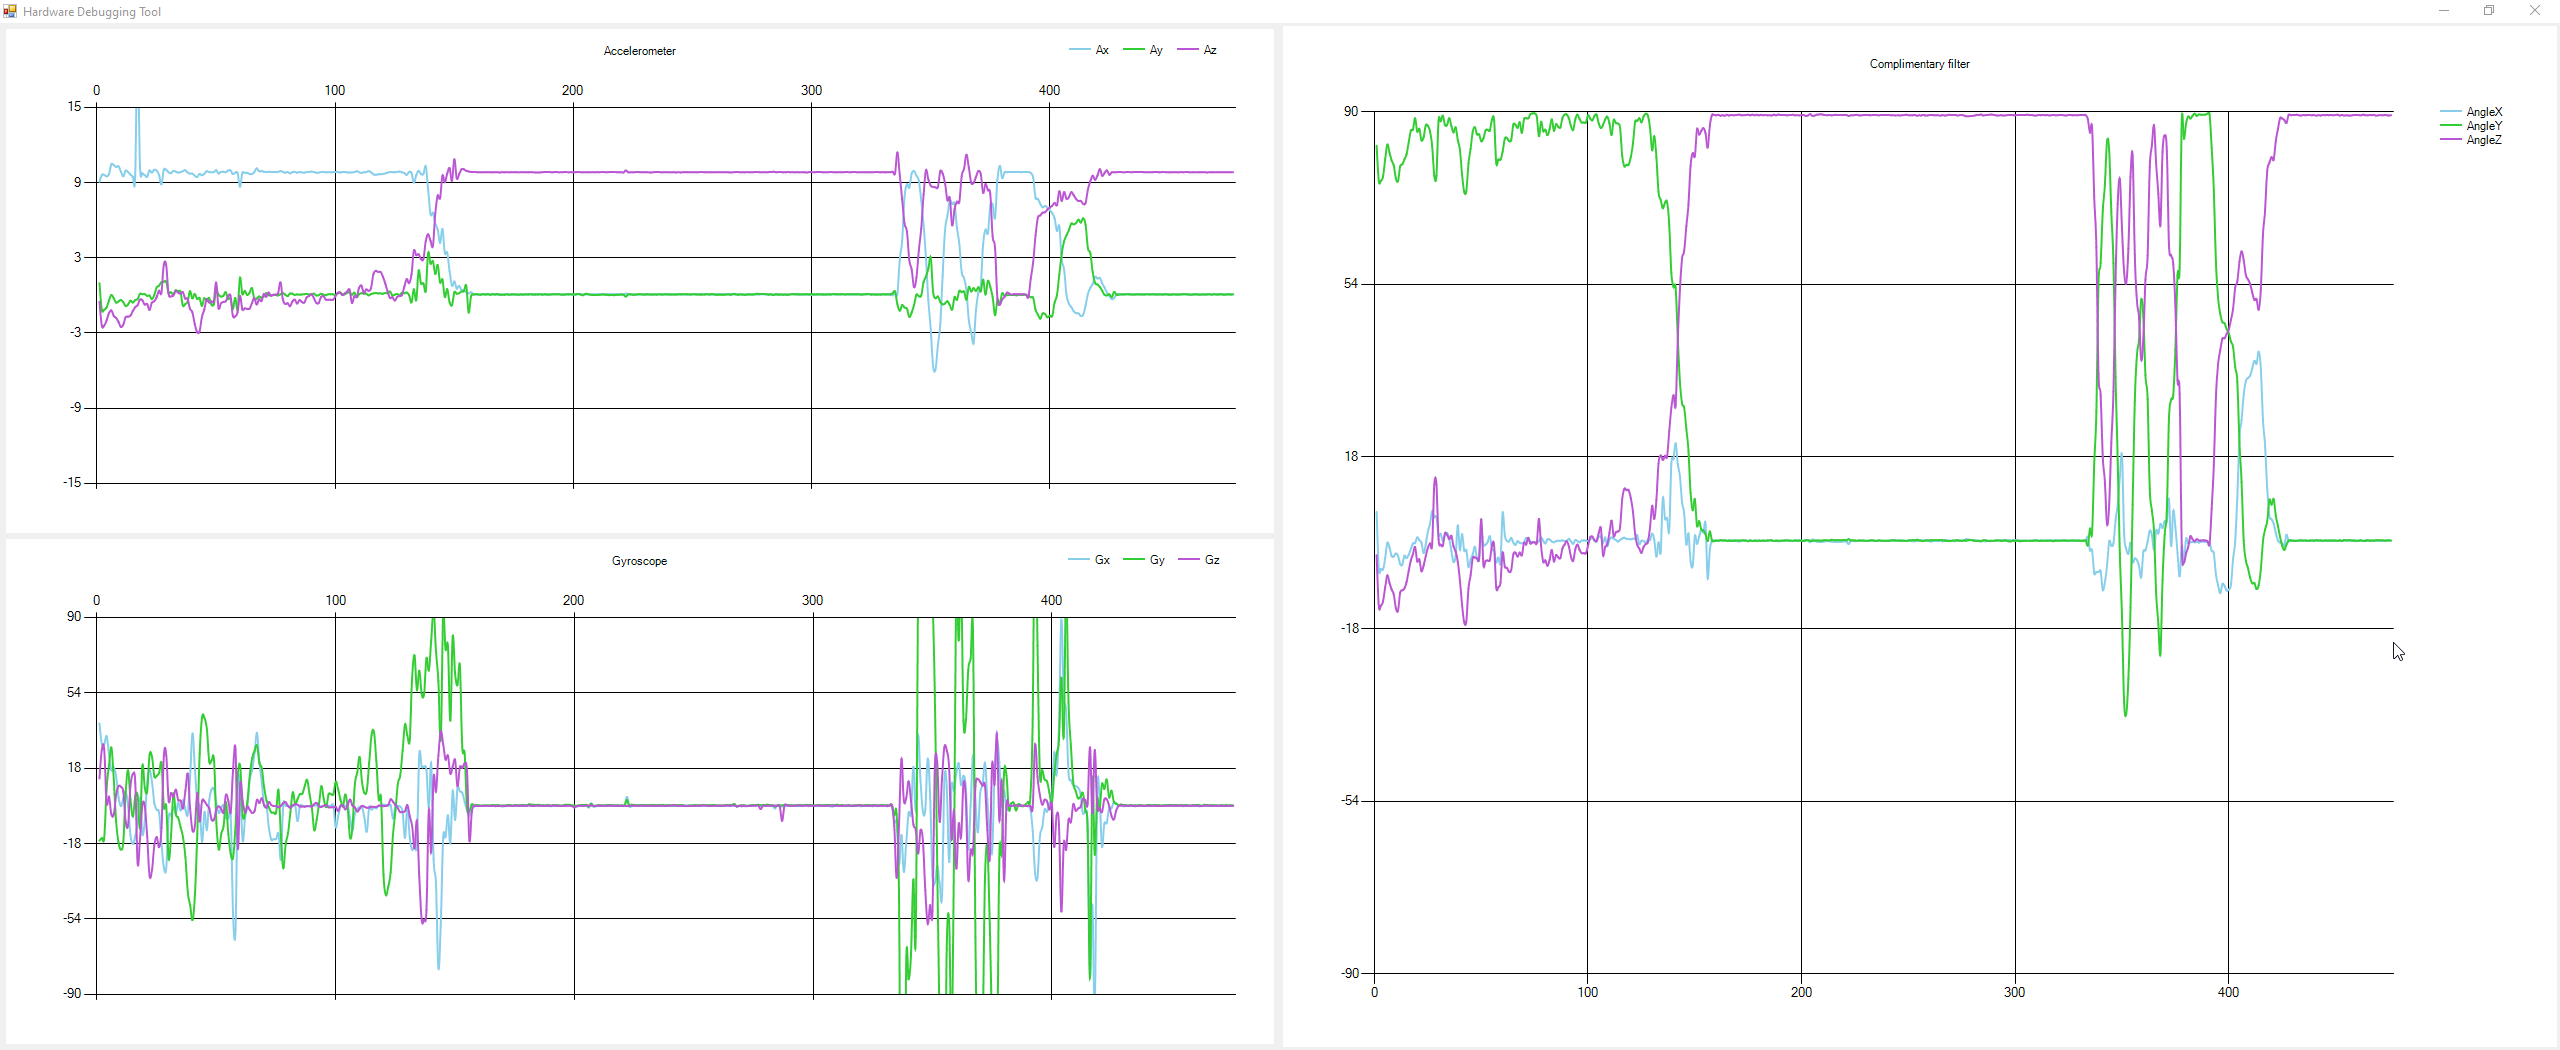
\includegraphics[width=\linewidth]{testen/GUI.png}
	\caption{Desktopapplicatie om Satellite te testen}
\end{figure}

\newpage
\subsection{LED's}
Er zitten standaard vier LED’s op het boordje, en ze hebben alle vier een andere kleur. De LED’s zijn puur voor de softwareontwikkelaar en zal door de kapitein van een binnenvaartschip niet gezien worden. Hieronder is gedefinieerd wanneer de LED’s gebruikt worden en waarvoor ze gebruikt worden \ref{tab:leds}. Er is voor errors en warnings de standaardkleuren rood en geel gebruikt. Daarnaast wordt ervoor het data ophalen een groen LED laten zien als dit succesvol is gedaan, bij fouten van het ophalen van de sensor data wordt een geel of rood LED getoond. Dit is gebaseerd hoe fout het is gegaan. Bij het versturen van sensor data of bij het ontvangen van data wordt er een blauw licht vertoont.
\begin{table}[h!]
	\caption{Satellite onboard LED beschrijving}
	\begin{tabular}{lp{14.5cm}}
	\toprule
	\textbf{LED Kleur} 	& \textbf{Beschrijving} \\ \toprule
	Groen	& Er wordt sensor data opgehaald\\
	Rood	& Error \\
	Blauw	& Data wordt opgestuurd, of data is ontvangen \\
	Geel	& Er is iets fout gegaan, Satellite probeert het op te lossen\\  \bottomrule
	\end{tabular}
	\label{tab:leds}
\end{table}